\begin{frame}
\frametitle{Логическое адресное пространство}
\begin{itemize}
    \item<1->Зачем вообще нужно разделение на логическое и
    физическое адресное пространства?
    \begin{itemize}
        \item<2->абстракция - приложение не знает о структуре
        физической памяти;
        \item<3->изоляция и защита - каждое приложение имеет
        свое логическое адресное пространство.
    \end{itemize}
\end{itemize}
\end{frame}

\begin{frame}
\frametitle{Понятие процесса}
\begin{itemize}
    \item<1->Процесс - контейнер для ресурсов ОС
    \begin{itemize}
        \item<2->ОС может и не поддерживать (XX-DOS);
        \item<3->ОС выделяет ресурсы, например, память, процессам;
        \item<4->код, исполняющийся в рамках процесса, используют его ресурсы.
    \end{itemize}
\end{itemize}
\end{frame}

\begin{frame}
\frametitle{Понятие процесса}
\begin{itemize}
    \item<1->Процессы, по-умолчанию, изолированны друг от друга:
    \begin{itemize}
        \item<2->у каждого процесса свое логическое адресное пространство;
        \item<3->т. е. код в рамках одного процесса не может залезть
        в память другого процесса.
    \end{itemize}
\end{itemize}
\end{frame}

\begin{frame}
\frametitle{Логическое адресное пространство}
\begin{itemize}
   \item<1->Как логические адреса отображаются на физические?
   \item<1->Как логические адресные пространства защищены?
   \begin{itemize}
       \item<2->сегментация (важно для x86);
       \item<3->paging (страничная организация памяти).
   \end{itemize}
\end{itemize}
\end{frame}

\begin{frame}
\frametitle{Сегментация}
\begin{itemize}
    \item<1->Сегментация в Real Mode:
    \begin{itemize}
        \item<2->логический адрес - сегмент ($SEG$) и смещение ($OFF$);
        \item<2->$SEG$ хранится в одном из сегментных регистров (\emph{CS},
        \emph{SS}, \emph{DS}, \emph{ES}, \emph{GS}, \emph{FS});
        \item<3->$A_{phys} = \left(SEG\times 16 + OFF\right)~mod~2^{20}$.
    \end{itemize}
\end{itemize}
\end{frame}

\begin{frame}
\frametitle{Сегментация}
\begin{itemize}
    \item<1->$SEG$ - идентификатор сегмента физической памяти:
    \begin{itemize}
        \item<2->сегмент $SEG$ начинается по физическому адресу $SEG\times 16$;
        \item<3->сегмент $SEG$ имеет размер $2^{16}$ байт.
    \end{itemize}
    \item<4->А что если разрешить ОС изменять параметры сегмента?
\end{itemize}
\end{frame}

\begin{frame}
\frametitle{Таблица дескрипторов сегментов}
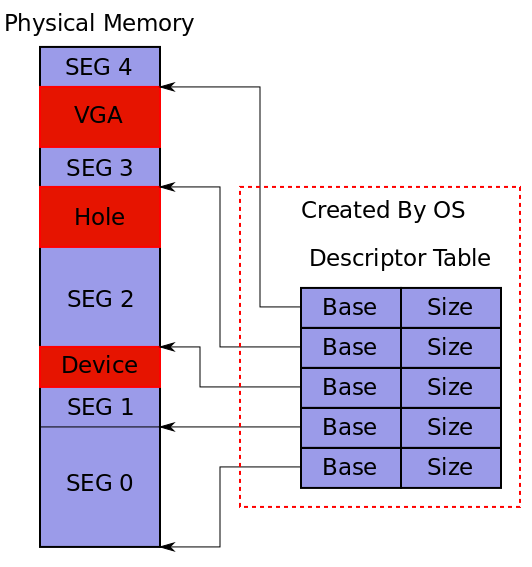
\includegraphics[height=.6\textheight]{dt}
\end{frame}

\begin{frame}
\frametitle{Изоляция и защита с помощью сегментации}
\begin{itemize}
    \item<1->Пусть ОС "выдает" каждому процессу свой дескриптор ($SEG$)
    \begin{itemize}
        \item<2->каждый дескриптор описывает свой участок физической памяти;
        \item<3->разные процессы пользуются разными дескрипторами (т. е. разные
        значения $SEG$);
        \item<4->непривилегированному коду запрещено изменять сегментные
        регистры.
    \end{itemize}
\end{itemize}
\end{frame}

\begin{frame}
\frametitle{Селектор сегмента}
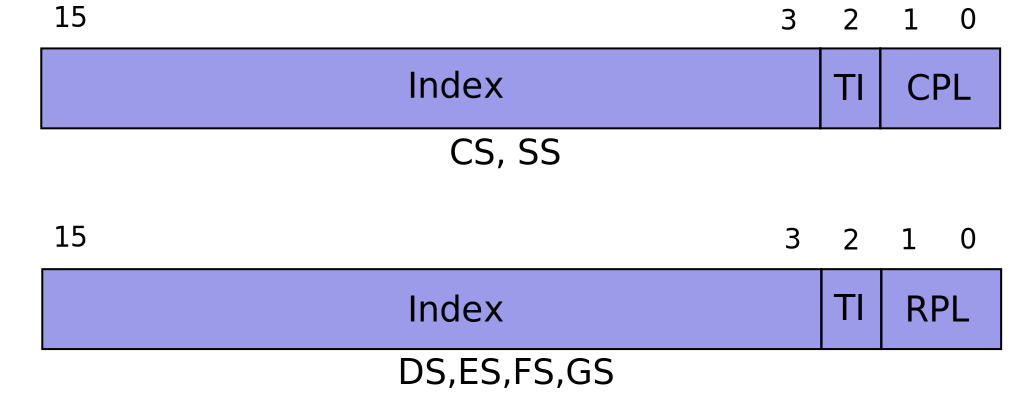
\includegraphics[height=.3\textheight]{sel}
\end{frame}

\begin{frame}
\frametitle{Уровни привелегий в x86}
\begin{itemize}
    \item<1->В x86 выделяют 4 уровня привилегий:
    \begin{itemize}
        \item<1->ring0 - ring3;
        \item<2->ring0 - наивысший уровень привилегий (пользовательские
        приложения);
        \item<2->ring3 - низший уровень привилегий (код ядра ОС).
    \end{itemize}
\end{itemize}
\end{frame}

\begin{frame}
\frametitle{Global Descriptor Table}
\begin{itemize}
    \item<1->В x86 таблицу дескрипторов называют GDT
    \begin{itemize}
        \item<2->адрес и размер GDT хранятся в специальном регистре GDTR;
        \item<3->писать и читать GDTR можно с помощью инструкций \emph{LIDT}
        и \emph{SIDT};
        \item<4->писать в GDTR может только привилегированный код.
    \end{itemize}
\end{itemize}
\end{frame}

\begin{frame}
\frametitle{Дескриптор сегмента в Protected Mode}
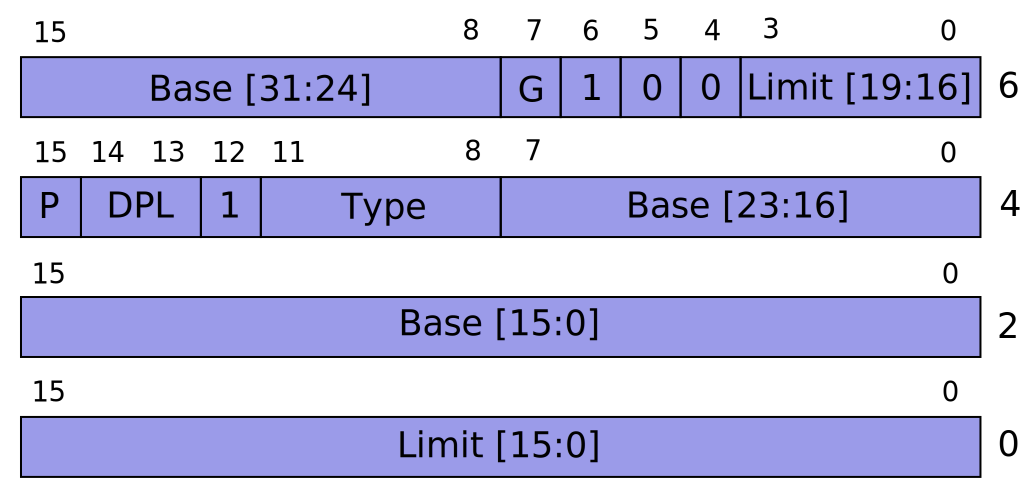
\includegraphics[height=.5\textheight]{gdt32}
\end{frame}

\begin{frame}
\frametitle{Преобразование в физический адрес}
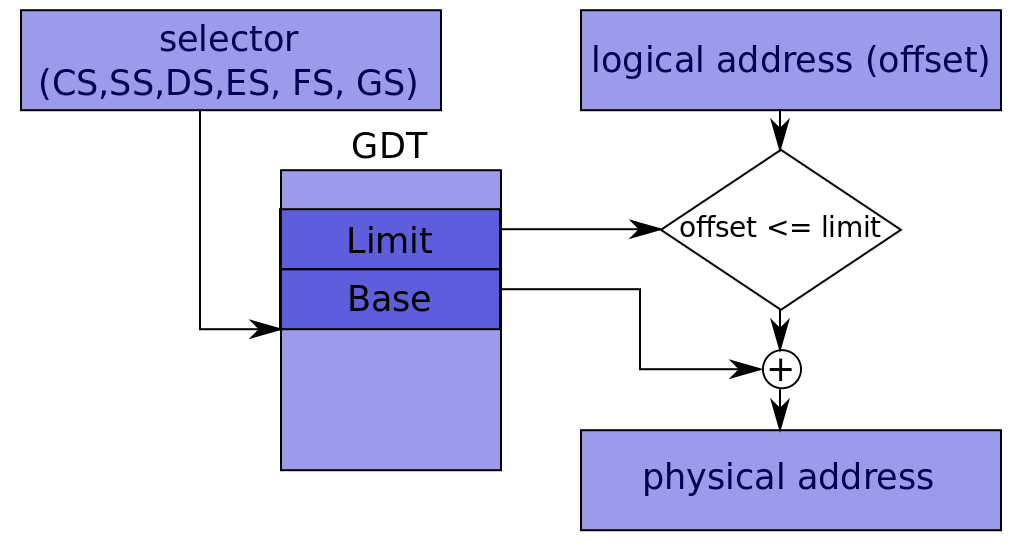
\includegraphics[height=.5\textheight]{gdttr}
\end{frame}

\begin{frame}
\frametitle{Сегментация в Long Mode}
\begin{itemize}
    \item<1->Сегментация в Long Mode \emph{практически} не используется
    \begin{itemize}
       \item<2->\emph{ES},\emph{DS},\emph{FS},\emph{GS} обычно равны 0;
       \item<3->поля \emph{Base} и \emph{Limit} дескрипторов игнорируются;
       \item<4->\emph{CS} и \emph{SS} все еще хранят \emph{CPL}.
    \end{itemize}
    \item<5->Вместо сегментации используется paging.
\end{itemize}
\end{frame}

\begin{frame}
\frametitle{Paging}
\begin{itemize}
    \item<1->Давайте просто использовать словарь
    \begin{itemize}
        \item<1->словарь хранит отображение логических адресов на физические;
        \item<2->ядро ОС создает свой словарь для каждого процесса.
    \end{itemize}
\end{itemize}
\end{frame}

\begin{frame}
\frametitle{Paging}
\begin{itemize}
    \item<1->Как должен выглядеть словарь?
    \begin{itemize}
        \item<2->отображать каждый байт отдельно непрактично;
        \item<3->отображение происходит блоками фиксированного размера
        (страницами);
        \item<4->размер страницы определяется архитектурой (типичные размеры:
        4Kb и 64Kb).
    \end{itemize}
\end{itemize}
\end{frame}

\begin{frame}
\frametitle{Paging}
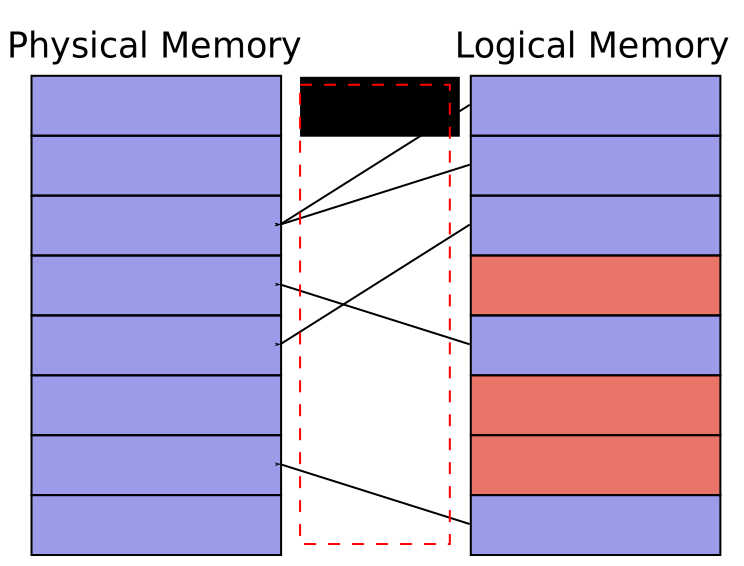
\includegraphics[height=.5\textheight]{pagemap}
\end{frame}

\begin{frame}
\frametitle{Paging}
\begin{itemize}
    \item<1->Как должен выглядеть словарь?
    \begin{itemize}
        \item<2->не каждый процесс использует все логическое адресное
        пространство (даже в 32-битных системах и тем более в 64-битных);
        \item<3->не хочется хранить информацию для неиспользуемых страниц;
        \item<4->структура должна быть сравнительно простой.
    \end{itemize}
\end{itemize}
\end{frame}

\begin{frame}
\frametitle{Таблица страниц}
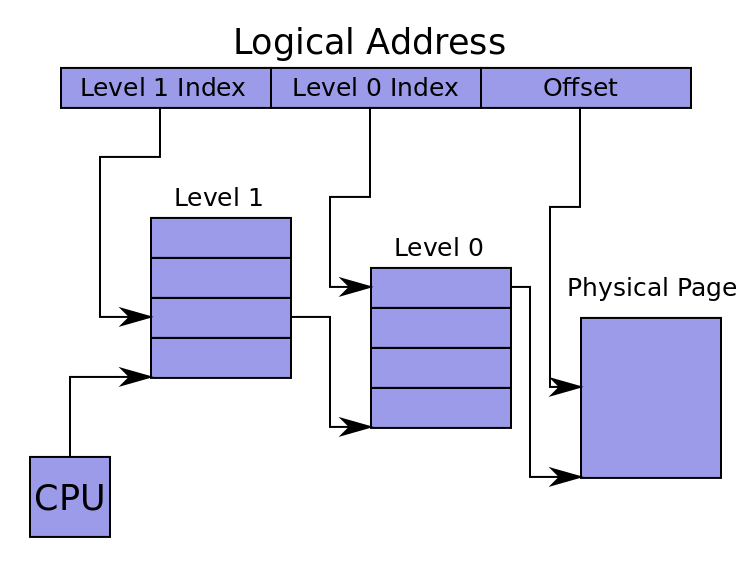
\includegraphics[height=.5\textheight]{pagetr}
\end{frame}

\begin{frame}
\frametitle{Translation Lookaside Buffer}
\begin{itemize}
    \item<1->А вы заметили проблему таблиц страниц?
    \begin{itemize}
        \item<2->мы хотим прочитать 1 байт по некоторому логическому адресу;
        \item<3->процессор должен прочитать записи в нескольких таблицах.
    \end{itemize}
\end{itemize}
\end{frame}

\begin{frame}
\frametitle{Translation Lookaside Buffer}
\begin{itemize}
    \item<1->Процессор кеширует результаты трансляции в TLB:
    \begin{itemize}
        \item<2->TLB может значительно ускорить обращение к памяти;
        \item<3->если код не обращается каждый раз к новой странице.
    \end{itemize}
\end{itemize}
\end{frame}

\begin{frame}
\frametitle{Translation Lookaside Buffer}
\begin{itemize}
    \item<1->Процессор не может отследить изменения в таблицах страниц:
    \begin{itemize}
        \item<2->TLB не прозрачен, т. е. необходимо явно "сбрасывать" записи;
        \item<3->об этом тоже должно заботиться ядро ОС.
    \end{itemize}
\end{itemize}
\end{frame}

\begin{frame}
\frametitle{Page Fault}
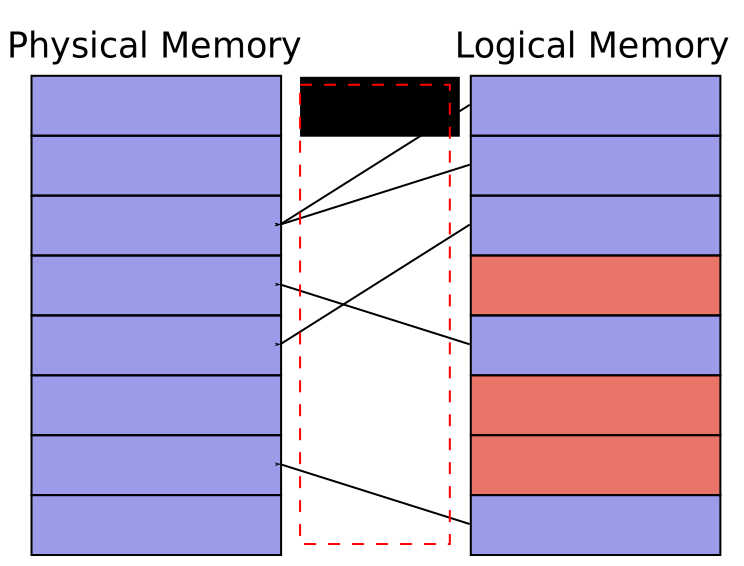
\includegraphics[height=.5\textheight]{pagemap}
\end{frame}

\begin{frame}
\frametitle{Page Fault}
\begin{itemize}
    \item<1->Не все записи в таблицах страниц используются
    \begin{itemize}
        \item<1->что, если код обратится к логическому адресу, для которого нет
        отображения?
        \item<2->генерируется специальное исключение - Page Fault.
    \end{itemize}
\end{itemize}
\end{frame}

\begin{frame}
\frametitle{Защита памяти}
\begin{itemize}
    \item<1->Paging также позволяет запретить некоторые действия с памятью:
    \begin{itemize}
        \item<2->мы уже видели запрет на обращение к памяти;
        \item<3->запись в какой-то участок логической памяти;
        \item<4->исполнение кода из какого-то участка памяти;
        \item<5->обращение непривилегированного кода.
    \end{itemize}
\end{itemize}
\end{frame}

\begin{frame}
\frametitle{Paging в x86 Long Mode}
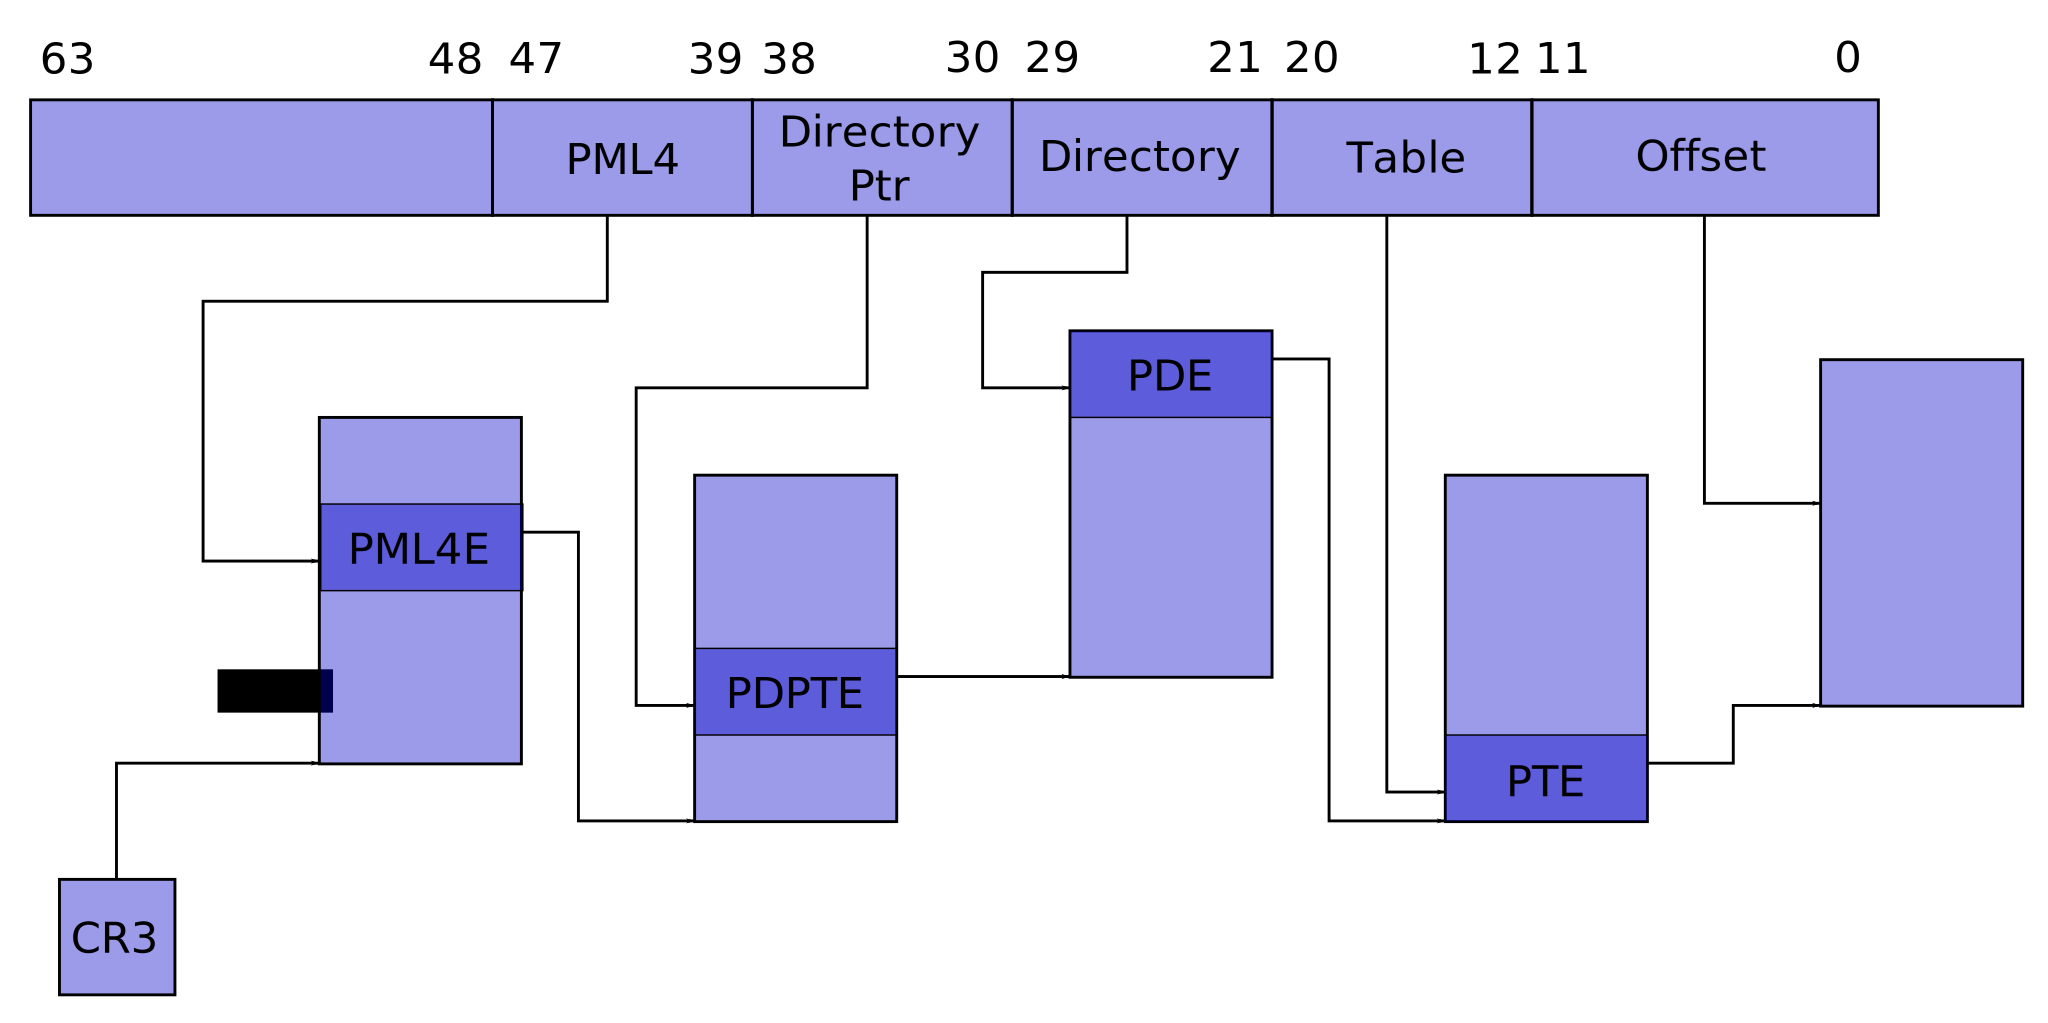
\includegraphics[height=.5\textheight]{pagex86}
\end{frame}

\begin{frame}
\frametitle{Paging в x86 Long Mode}
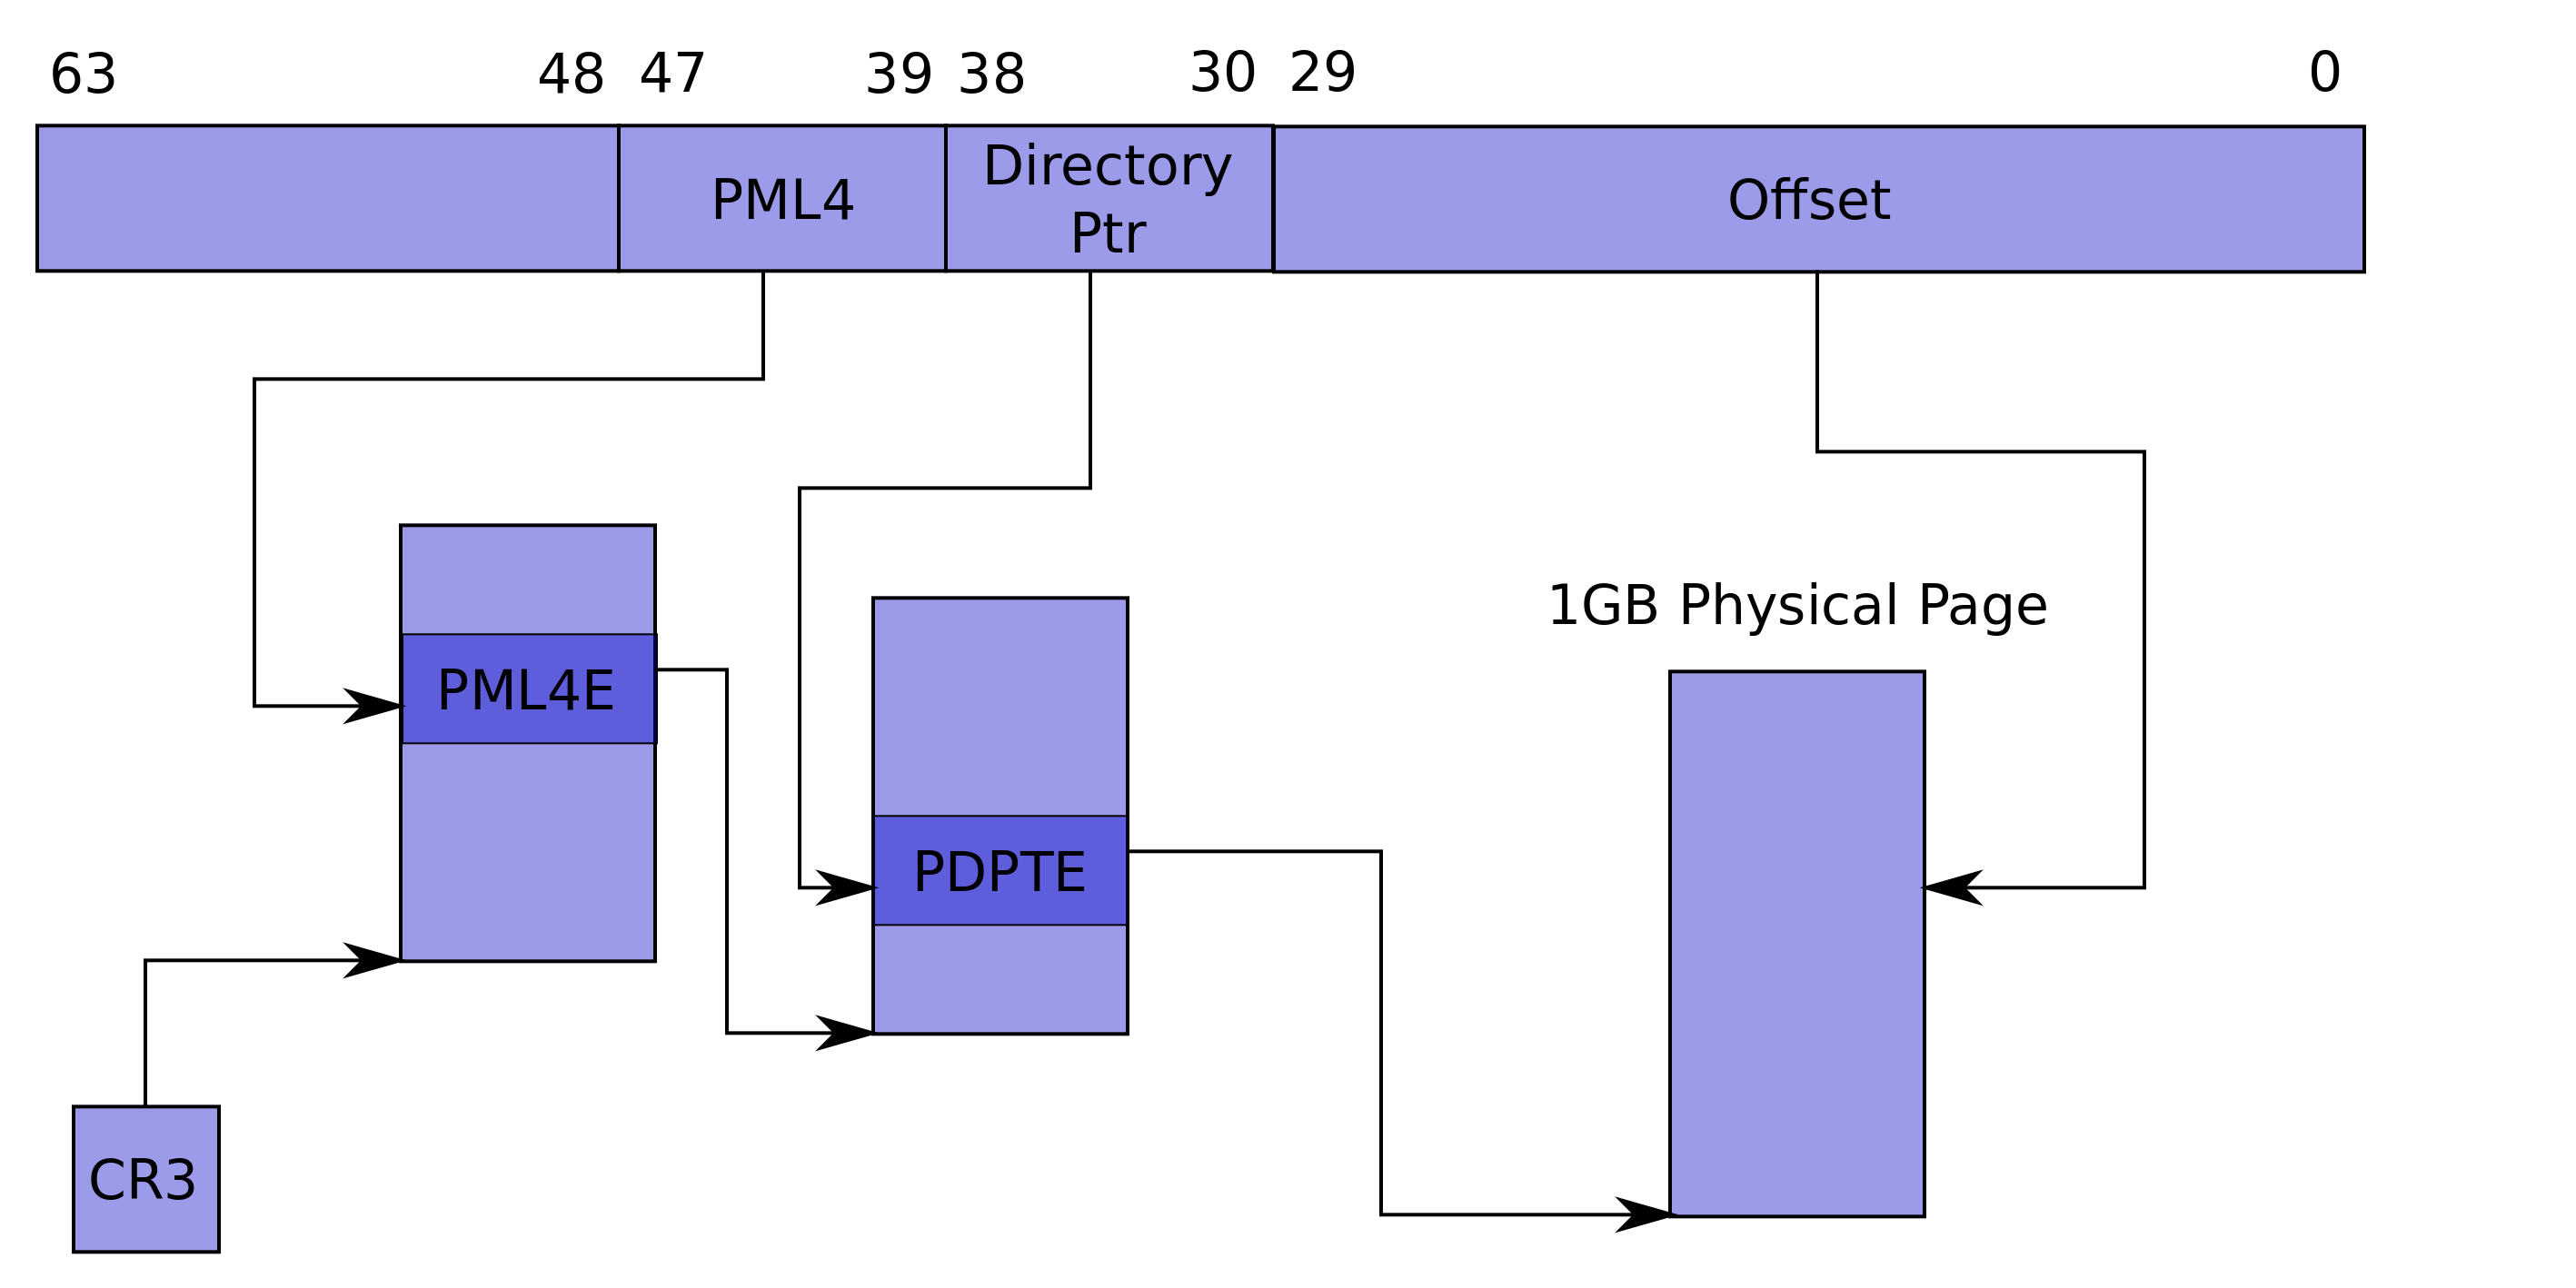
\includegraphics[height=.5\textheight]{page1gb}
\end{frame}

\begin{frame}
\frametitle{Paging в x86 Long Mode}
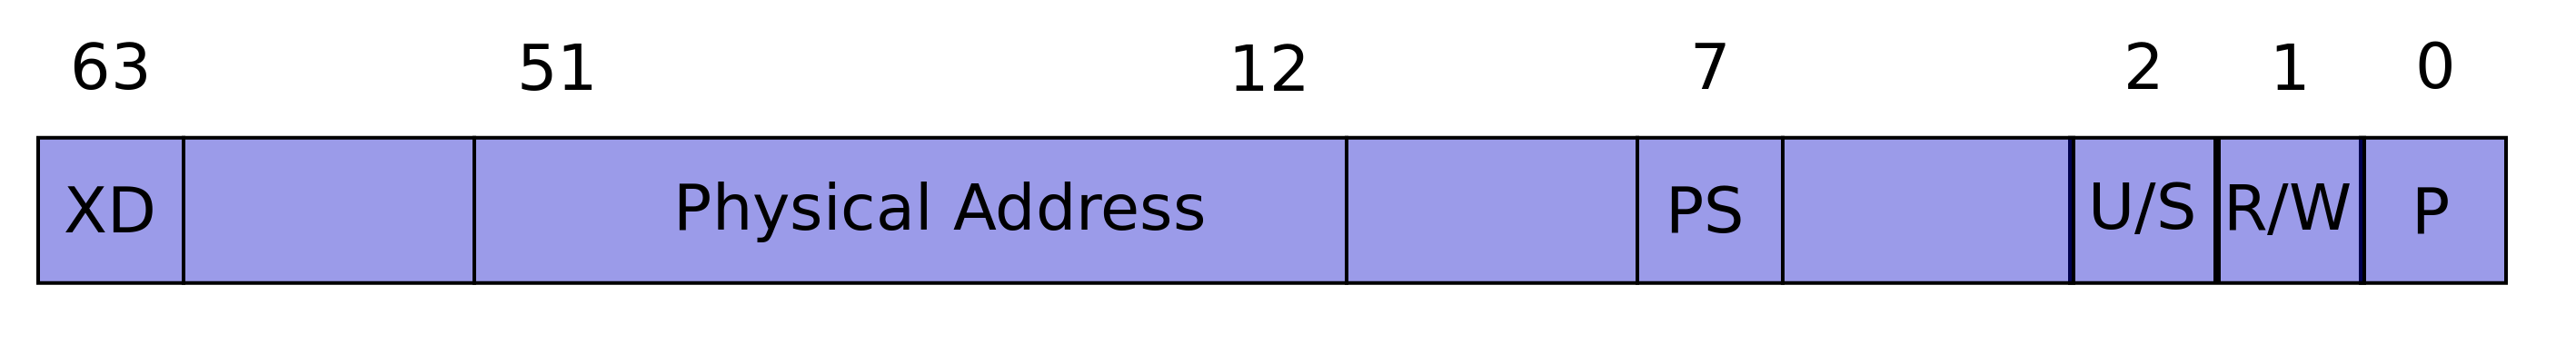
\includegraphics[height=.13\textheight]{pte}
\begin{itemize}
    \item\emph{P} - если 0, запись не используется;
    \item\emph{R/W} - если 0, то запись запрещена;
    \item\emph{U/S} - если 0, то запрещен непривилегированный доступ;
    \item\emph{PS} - если 1, это последний уровень;
    \item\emph{XD} - если 1, то запрещено исполнение.
\end{itemize}
\end{frame}

\begin{frame}
\frametitle{Резюме}
\begin{itemize}
    \item<1->Логическое и физическое адресное пространства:
    \begin{itemize}
        \item<2->программы используют логические адреса (указатели);
        \item<3->процессор использует физические адреса;
        \item<4->ОС определяет как логические адреса отображаются на физические.
    \end{itemize}
\end{itemize}
\end{frame}

\begin{frame}
\frametitle{Резюме}
\begin{itemize}
    \item<1->Понятие процесса:
    \begin{itemize}
        \item<2->каждый процесс имеет свое логические адресное пространство;
        \item<3->процессы изолированы друг от друга.
    \end{itemize}
\end{itemize}
\end{frame}

\begin{frame}
\frametitle{Резюме}
\begin{itemize}
    \item<1->Сегментация и страничная адресация памяти:
    \begin{itemize}
        \item<2->ОС использует эти аппаратные механизмы для организации изоляции
        процессов;
        \item<3->многие современные архитектуры с поддержкой защиты памяти
        используют paging (и очень немногие сегментацию).
    \end{itemize}
\end{itemize}
\end{frame}
